\begin{marginfigure}
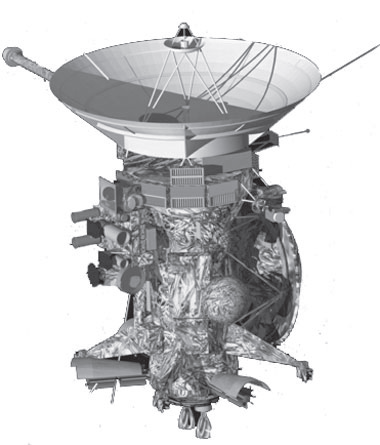
\includegraphics[width=\linewidth]{fig_00}
\end{marginfigure}

%\subsection*{Activité préparatoire : Génération d'une grille -- Déjà fait sur Capytale}


\section*{Résolution du labyrinthe}

Il est possible de résoudre le labyrinthe en utilisant un parcours en largeur ou un parcours en profondeur.

\begin{question} Écrire la fonction \lstinline{resolution_largeur(G:dict, s:tuple) -> list} qui permet de résoudre le labyrinthe en utilisant un parcours en largeur. Cette fonction renvoie la liste des sommets permettant d’atteindre le sommet en haut à droite depuis le sommet en bas à gauche.
\end{question}

\begin{question}
Afficher en trait épais bleu la solution donnée par le parcours en largeur.
\end{question}

\begin{question}
Répondre aux mêmes questions en utilisant un parcours en profondeur.
\end{question}


